\documentclass{article}
\usepackage[utf8]{inputenc}
\usepackage[russian]{babel}
\usepackage{graphicx}
\usepackage{amsmath}
\usepackage{breqn}
\usepackage{wrapfig}
\usepackage{float}
\usepackage{multirow}
\usepackage{caption}
\usepackage{subcaption}

\graphicspath{ {./data/images} }
\author{Александр Романов Б01-107}
\date{}
\title{4.1.1 Изучение центрированных оптических систем}

\begin{document}
\maketitle
\section{Введение}
\subsection{Цель работы}
изучить методы определения фокусных расстояний линз и сложных оптических систем; определить
характеристики оптической системы, составленной из тонких линз; изучить недостатки реальных линз
-- сферическую и хроматическую аберрации.
\subsection{В работе используются}
оптическая скамья с набором рейтеров, положительные и отрицательные линзы, экран, осветитель с
ирисовой диафрагмой, зрительная труба, светофильтры, кольцевые диафрагмы, линейка.
\section{Работа}
\section{Центрировка оптической системы}
Из имеющегося набора отберём собирающие линзы. Для этого держа линзу в одной руке, получим на ладони
другой руки изображение изображение удалённой лампы. Таким же образом определим их приблизительные
фокусные расстояния.

\begin{figure}[H]
  \centering
  \begin{tabular}{|c|c|c|c|}
    \hline
    Л1 & Л2 & Л3 & Л4 \\\hline    
    \(F = 9.5\pm 0.5\;cm\)&\(F = 12.5\pm 0.5\;cm\)&\(F = 11.5\pm 0.5\;cm\)& рассеивающая\\\hline
  \end{tabular}
\end{figure}

На одном конце оптической скамьи установим осветитель со стрелкой и вплотну. к нему - экран на рейтере.
Отрегулируем высоту так, чтобы его центр совпадал с центром яркого пятна от осветителя.

Отцентрируем собирающую линзу. Для этого отодвинем экран от осветителя и разместим в промежутке рейтер
с собирающей линзой Л1. Передвигая линзу и экран вдоль скамьи получим на экране чёткое изображение
предмета-стрелки. Закрепим рейтеры. Смещая линзу с помощью поперечных саазок и по высоте, приведём изображение
к центру экрана.

Отцентрируем все положительные линзы, добавляя их к системе последовательно (не убирая уже отцентрированные).

\subsection{Определение фокусных расстояний тонких линз при помощи экрана}
Воспользуемся методом Аббе.
\begin{figure}[H]
  \centering
  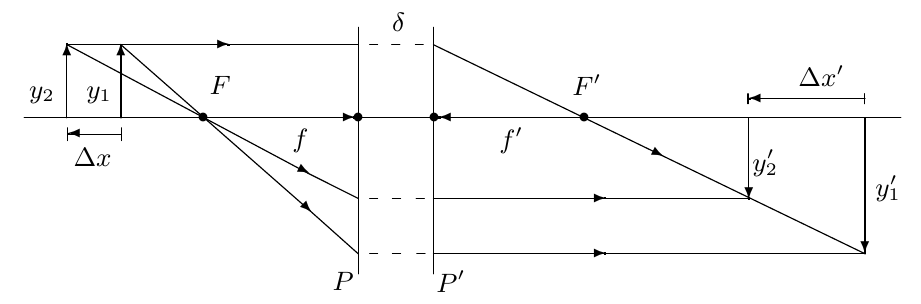
\includegraphics[width = \textwidth]{Abbe.png}
  \caption{Схема для метода Аббе}
\end{figure}

Закрепим собирающую линзу Л1 между осветителем и экраном. Перемещая осветительвдоль скамьи, получим на
экране резкое изображение предета при двух различных положений источника и экрана. Результаты (\(y_0 = 1\; cm\)):

\begin{figure}[H]
  \centering
  \begin{tabular}{|c|c|c|c|}
    \hline
    № & a, cm    & b, cm    & y1, cm\\\hline
    1 & \(20 \pm 1\) & \(44 \pm 1\) & \(1.5\pm 0.1\) \\\hline
    2 & \(13 \pm 1\) & \(112 \pm 1\) & \(9\pm 0.1\) \\\hline
  \end{tabular}
\end{figure}

Отсюда получим фокусное расстояние:
\[ F_1 = \frac{a_2 - a_1}{y_0/y_2 - y_0/y_1} = (12.6 \pm 1.0)\; cm \]
\[ F_1 = \frac{b_2 - b_1}{y_2/y_0 - y_1/y_0} = (9.0 \pm 1.0)\; cm \]

Второй результат кажется более правдоподобным, т.к. близко совпдает с измеренным до этого. Неточность
первого можно объяснить неточностю измерения расстояния \(a\).

Определим фокусное расстояние отрицательной линзы. Сначала с помощью Л1 получим на экране
увеличенное изображение предмета и измерим расстояние от центра линзы до экрана (\(a = 19\pm1\; cm\)). Затем
между собирающей линзой и экраном разместим рассеивающую линзу и, отодвигая экран от линзы, найдём 
действительное изображение предмета, образованного системой линз.
Измерим расстояние от рассеивающей линзы до экрана (\(b = 55 \pm 1\; cm\)) и расстояние между линзами 
(\(l = 27 \pm 1\; cm\)). Отсюда определим фокусное расстояние линзы Л4:
\[ \frac{1}{F_4} = \frac{1}{b} - \frac{1}{a-l} \Rightarrow F_4 = (6.9\pm 0.5)\;cm\]


\subsection{Опрежеление фокусных расстояний тонких линз с помощью зрительной трубы}
Настроим трубу на бесконечность. Поставим собирающую линзу Л1 на расстоянии от предмета примерно равном
фокусному. На небольшом расстоянии от линзызакрпим трубу, настроенную на бесконечность и
отцентрируем её по высоте. Передвигая линзу вдоль скамьи, получим в окуляре зрительной трубы чёткое
изображение предмета. При этом расстояние между предметом и сереиной тонкой линзы равно фокусному.
Получим рзначение
\[ F_1 = (9.5\pm 0.5)\; cm\]

Проделаем то же самое для Л2:
\[ F_2 = (13.0\pm 0.5)\; cm\]

Для определения фокусного расстояния рассеивающей линзы используем схему на Рис.\ref{fig:dispel}
\begin{figure}[H]
  \centering
  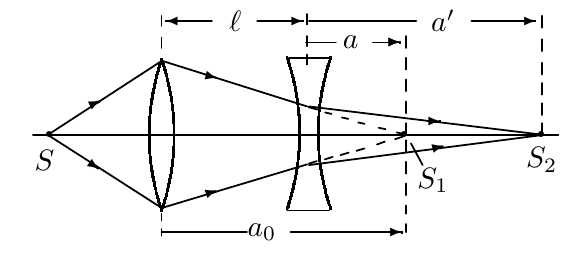
\includegraphics[width = \textwidth]{dispel.png}
  \caption{Измерение фокусного расстояния рассеивающей линзы}\label{fig:dispel}
\end{figure}

Сначала получим на экране увеличенное изображение предмета с помощью Л2. Измерим расстояние
между линзой и экраном (\(a_0 = 35\pm 0.5\; cm\)). Разместим сразу за экраном трубу,
настроенную на бесконечность, и закрепим её. Уберём экран и поставим на его место исследуемую
рассеивающую линзу Л4. Отцентрируем световой пучок. Перемещая рассеивающую линзу, найдём в 
окуляре зрительной трубы резкое изображение предмета. Измерив расстояние между линзами
(\(l = 30 \pm 1\; cm\)), найдём фокусное расстояние рассеивающей линзы:
\[ F_4 = l - a_0 = (5.0 \pm 0.5)\; cm \]

Сведём результаты всех измерений фокусных расстояний в одну таблицу:
\begin{figure}[H]
  \centering
  \begin{tabular}{|c|c|c|c|c|}
    \hline
    Способ & F_1, cm & F_2, cm & F_3, cm & F_4, cm \\\hline
    Проецируя изображение на ладонь   & \(9.5 \pm 0.5\) & \(12.5 \pm 0.5\) & \(11.5\pm 0.5\) & - \\\hline
    Аббе     & \(9.0 \pm 1.0\) & - & - &\(6.9 \pm 0.5\) \\\hline
    Зрительная труба & \(9.5 \pm 0.5\) & \(13.0 \pm 0.5\) & - &\(5 \pm 0.5\) \\\hline
  \end{tabular}
\end{figure}

Все результаты довольно близко совпдают друг с другом. Значения, полученные методом Аббе,
вызывают больше всего сомнений. Это может быть связано с неточностью измерения расстояния и тем
что в ходе эксперимента было тяжело понять в какой момент изображение достигает наибольшей чёткости.

\subsection{Определение фокусного расстояния и положения главных и фокаьных плоскостей сложной оптической системы}
Для создания сложной оптической системы установим в центре оптической скамьи две тонкие собирающие линзы
Л1 и Л2, сблизив их на минимально возможное расстояние. Закрепим рейтеры и измерим расстояние между
центрами линз (\(l_{12} = 4.5 \pm 0.5\; cm\)).

Для определения фокусного расстояния системы методом Абе расположим экран на дальнем конце скамьи.
Перемещая осветитель вдоль скамьи, получим на экране резкое изображение предмета. Измерим расстояние от
предмета до первой линзы и величину изображения (\(y_1 = 4.7\pm 0.1\; cm\)).
Передвинем источник на \(\Delta x = 1 \pm 0.5 \;cm\). При этом изображение передвинется на \(\Delta x' = 49 \pm 1\; cm\).
Изображение достигнет размера \(y_2 = 11.3\pm 0.1\; cm \). Вычислим фокусное расстояние системы:
\[F_{2\Sigma} = \frac{\Delta x}{y_0/y_1 - y_0/y_2} = 8\pm 1.0\; cm \]
\[F_{2\Sigma} = -\frac{\Delta x'}{y_1/y_0 - y_2/y_0} = 7.4 \pm 1.0\; cm\]
Результаты совпадают в пределах погрешности. При этом:
\[ -\frac{1}{F_{2\Sigma}} = \frac{1}{f_1} + \frac{1}{f_2} - \frac{l_{12}}{f_1f_2} \Rightarrow F_{2\Sigma} = 6.8 \pm 0.8\; cm\]
Результат близок к полученному выше.

Для нахождения положений главных фокусов систему уберём экран, закрепим зрительную трубу за второй
линзой, пододвинем осветитель к первой линзе и отцентрируем систему.
Медленно отодвигая осветитель от система, сначала найдём резкое изображение поверхности стекла в
окуляре зрительной трубы, а затем, последовательно уменьшая размер пятна и перемещая пятно в помощью винта
поперечных салазок линзы, настроимся на изображение предмета. Определим положение переднего главного
фокуса системы относительно первой линзы, измерив расстояние от этой линзы до предмета:
\[ F_{1\Sigma} = 3.0 \pm 0.5\; cm \]

Поменяем линзы местами, сохранив неизменныс растояние между их центрами и повторим измерения, тем самым
определив положение второго главного фокуса системы:
\[ F_{2\Sigma} = 6.0 \pm 0.5\; cm \]

\begin{figure}[H]
  \centering
  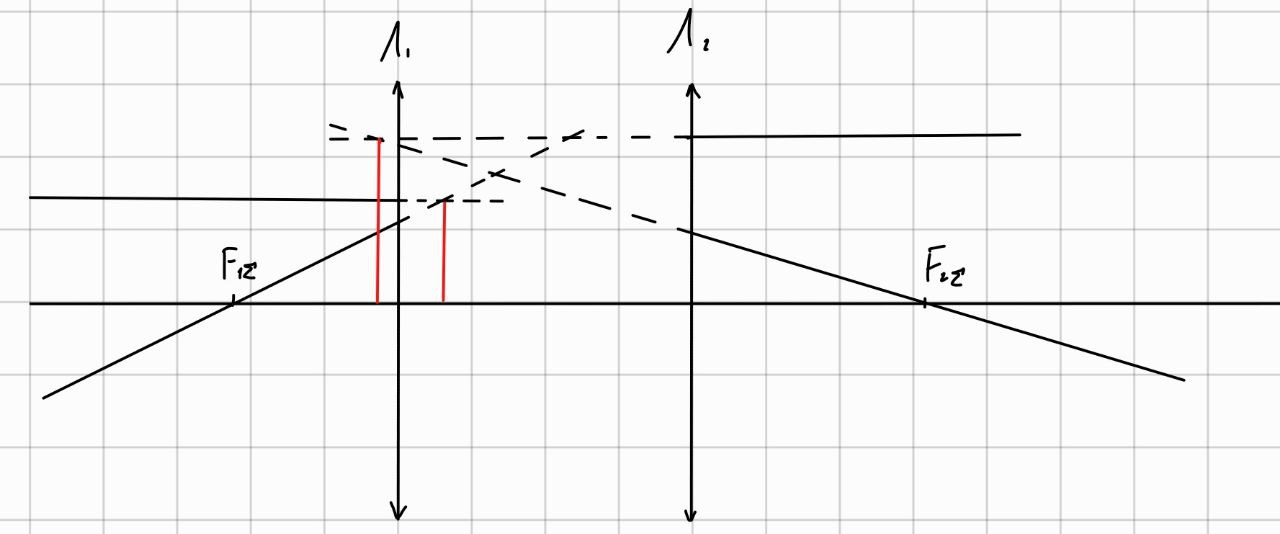
\includegraphics[width=\textwidth]{draw.jpeg}
  \caption{Чертёж оптической системы}\label{fig:draw}
\end{figure}

\subsection*{А. Основные аберрации оптических систем}
\subsection{Сферическая аберрация}
Для качественного наблюдения сферической аберрации расположим осветитель и экран на дальних концах
скамьи. Установите плосковыпуклую линзу Л3 на расстоянии \(a_1 = 11\;cm\). Наденем на неё маску
минимального размера (диафрагму диаметром \(2h = 1\;cm\)). Перемещая линзу, получим на удалённом
экране резкое изображение предмета. Расстояние от линзы до изображения:
\[ a_1' = 110 \pm 1\; cm \]

Установим маску максимального диаметра (\(2h = 4\;cm\)), передвигая экран снова получим резкое
изображение предмета. Расстояние от линзы до изображения:
\[ a_2' = 94 \pm 1\; cm\]

Заметим, что расстояние от линзы до изображения сильно изменилось. Это и есть проявление аберрации.
% \subsection{Хроматическая аберрация}
% Используя зрительную трубу и три светофильтра (красный, жёлтый и синий), определим по нониусной
% шкале положения плосковыпуклой линзы, соответствующие резкому изображения предмета. Фильтры 
% будем располагатьв параллельном пучке (За окуляром зрительной трубы), чтобы они не изменяли
% хода лучей.
% Фокусное расстояние \(F_3\) линзы Л3, измеренное с жёлтым фильтром

\section{Выводы}
В результате выполнения работы:
\begin{enumerate}
  \item Были изучены способы измерения фокусного расстояния линз и оптической системы.
  \item Были измерены фокусные расстояния наших линз несколькими способами: 
  \begin{figure}[H]
    \centering
    \begin{tabular}{|c|c|c|c|c|}
      \hline
      Способ & F_1, cm & F_2, cm & F_3, cm & F_4, cm \\\hline
      Проецируя изображение на ладонь   & \(9.5 \pm 0.5\) & \(12.5 \pm 0.5\) & \(11.5\pm 0.5\) & - \\\hline
      Аббе     & \(9.0 \pm 1.0\) & - & - &\(6.9 \pm 0.5\) \\\hline
      Зрительная труба & \(9.5 \pm 0.5\) & \(13.0 \pm 0.5\) & - &\(5 \pm 0.5\) \\\hline
    \end{tabular}
  \end{figure}
  \item Было проведено наблюдение эффекта оптических аберраций.
\end{enumerate}
\end{document}